\section{Method}


\begin{figure}
      \centering
      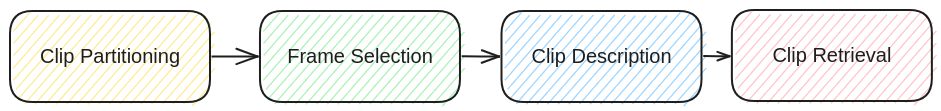
\includegraphics[width=0.8\textwidth]{figures/pipeline.png}
      \caption{High level block diagram of the proposed video understanding pipeline.}
      \label{fig:pipeline}
\end{figure}

The proposed pipeline is designed in such a way to be general to different video understanding tasks, with each of the 4 major steps allowing for multiple methods, or being optional for some tasks.
For the purposes of this work, a "clip" is a small segment of a video that is a few seconds long, 
and is highly cohesive in what it depicts. For example, in a movie, a clip might be a single shot.
At a high level, the pipeline for video understanding using LLMs is as follows:
\begin{enumerate}
      \item Partition the video into individual clips (optional)
      \item From each clip, select a small subset of frames to represent the clip
      \item Using the selected frames, generate a textual description of the clip using an LLM.
      \item Using the textual description, answer queries about the video, or retrieve clips.
\end{enumerate}

For brevity, these steps will be referred to as "Clip partitioning", "Frame selection", "Clip description", and "Clip Retrieval" respectively.
The two most applicable tasks for this pipeline are video retrieval and video summarization.
In video retrieval, given a query, the goal is to retrieve the video in a video dataset that best matches the query.
In visual video summarization, the goal is to edit a video down to a shorter length, containing only clips relevant to a given query.
Prior works often treat the video as-is and do not pre-process it much.



\section{Clip Partitioning}

Videos can contain a lot of different clips, which may or may not be related.
As such, it's desirable to process and describe each clip individually; clips are an atomic unit in video.
The input for clip partitioning is the whole video, and the output is a list of breaks (frame numbers) between clips.
The difficult aspect of clip partitioning is to efficiently find the boundaries between clips.
A two-hour video at 24 frames per second contains 172,800 frames, and so processing each one is computationally expensive.

The simplest approach to clip partitioning is to simply partition the video into equal-sized clips, without regard for the content of the video.
This approach is simple and fast to compute, but the resulting clips are not necessarily cohesive, since "clips" could contain multiple scenes and shots.

\subsection{Coarse-to-fine clip partitioning}
A more strategic approach identifies breaks as sequential frames with a large difference between them.
However, even computing a simple difference such as an L1 or L2 norm between each pair of frames is computationally expensive, since a norm must be taken per frame in the video.

As such, the VideoDescriptor pipeline uses a coarse-to-fine approach to clip partitioning.
The algorithm starts by computing the L1 distance between frames \textit{1 second apart}, over the entire video.
If the the L1 distance between these frames is above a certain threshold, then its likely that there's a clip break between them.
Thus, the 1-second segment is evaluated frame by frame, and if the distance between two frames is above the threshold, then a clip break is identified.
Empirically, this approach saves 60\% of the L1 computations compared to the naive frame-by-frame approach, and could save more if fewer coarse breaks are identified.

See Figure \ref{fig:breaks} for resulting clip breaks from the coarse-to-fine approach.
Qualitative results show that this approach is very effective at identifying clip breaks, with few false positives and false negatives.

\begin{figure}
      \centering
      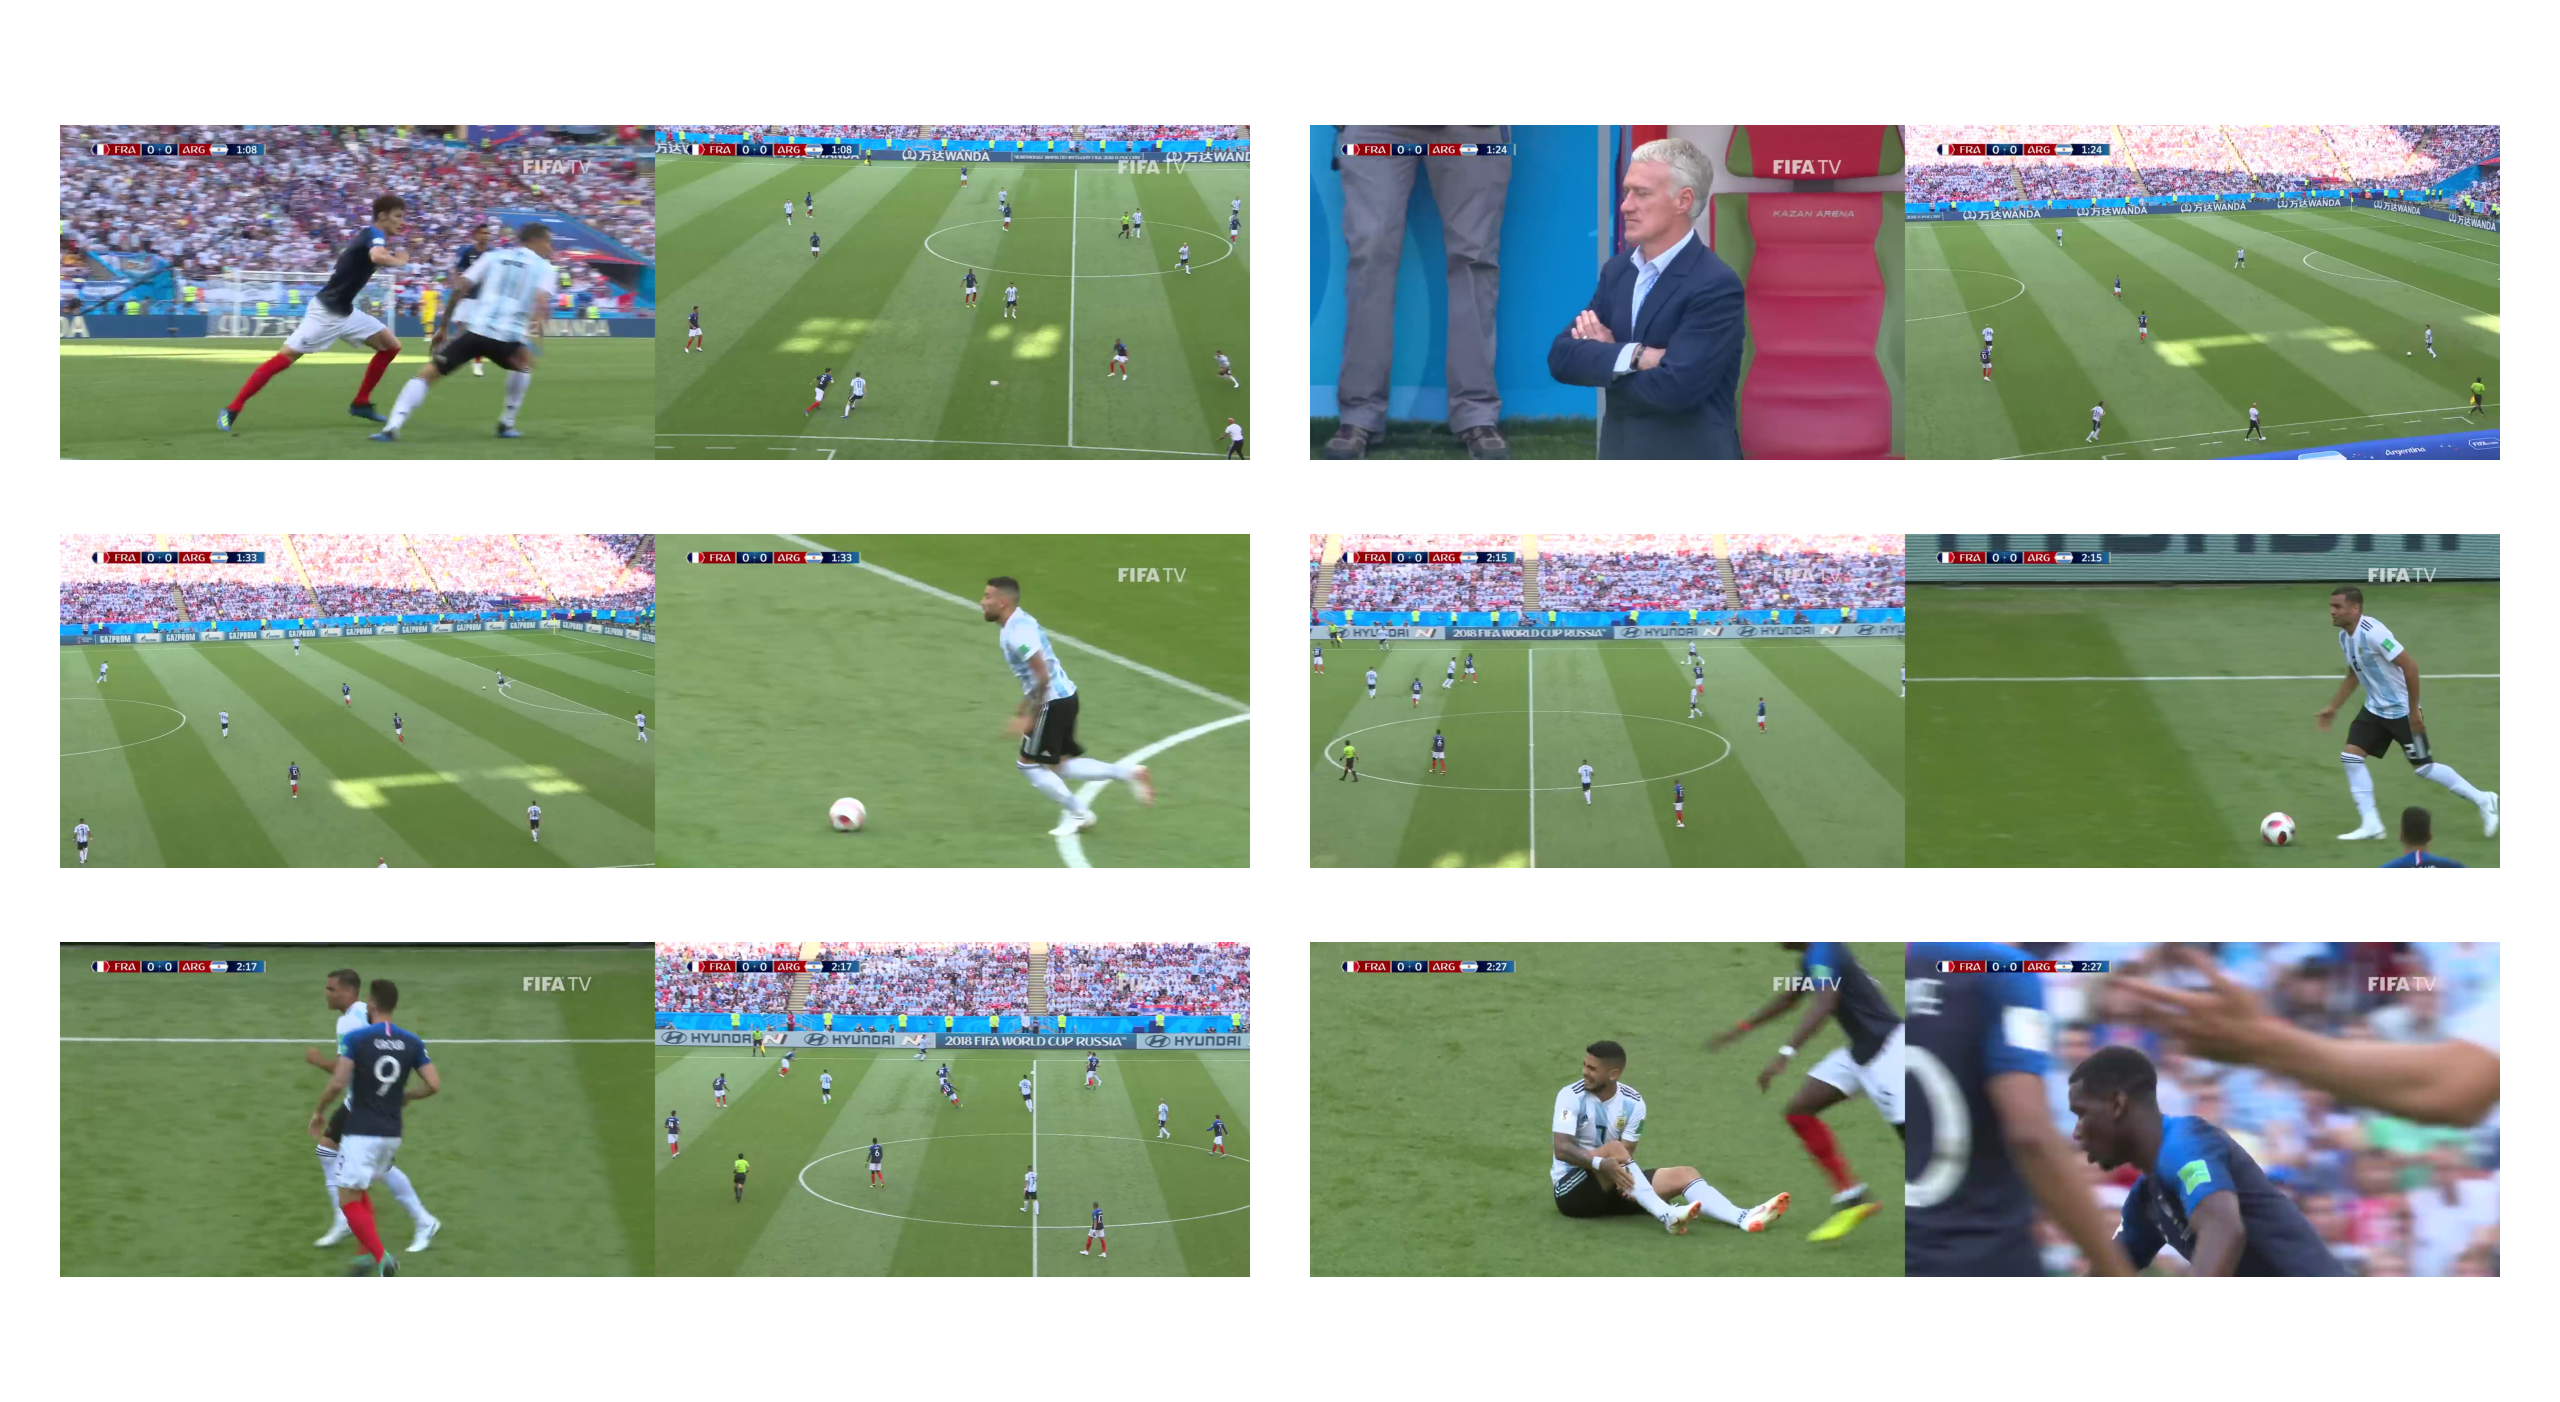
\includegraphics[width=\textwidth]{figures/breaks.png}
      \caption{Frames immediately before and after a clip break, determined by the coarse-to-fine clip partitioning strategy.}
      \label{fig:breaks}
\end{figure}


\section{Frame Selection}

Even within a single clip, there are a lot of frames, most of which are very similar to their neighbours.
To make the pipeline efficient, it's critical to select the subset of the most semantically relevant frames.
While some LLMs like LLaVA can take multiple images as input, they are rarely tested and likely not trained on multi-image inputs.
The input to frame selection is a clip (small length of video) and the output is a list of frames selected for further processing.

Earlier works simply sample randomly \cite{clipbert} or sample uniformly, at a course framerate such as 1 frame per second \cite{clip4clip}.

This work explores 3 different frame selection strategies:
greedy L1 selection, stratified sampling, random sampling, and stratified triplet sampling.

\subsection{Stratified Sampling}
To get a potentially more diverse set of frames, the first, last and middle frames are selected.
For brevity, this sampling method is referred to as \verb|3strat|. \verb|5strat| is also explored, which selects the first, last, and 3 evenly spaced frames in between.

\subsection{Random Sampling}
A random sampling approach is also explored, with either 3 or 5 frames selected from the video (with replacement).
These are referred to as \verb|3rand| and \verb|5rand| respectively.

\subsection{Stratified Triplet Sampling}
It's possible that the stratified sampling method above is too coarse, and that a single frames at multiple points in the clip is not enough to capture the clip's content.
For this reason, this work also explores stratified triplet sampling, where at each of the 3 points in the clip, 3 frames are selected across 1 second.
The motivation for this method is that the 3 frames in a single second will show what is changing in the scene.
each triplet is fed in as a single input into the LLM, which can take multiple images as input.
As a result, there is only one textual description per triplet in this sampling method.

\subsection{Greedy L1 Selection}
Greedy L1 selection initially selects the first frame of a clip. Then, it selects an additional clip if the L1 distance between the new frame and the previously selected frame is greater than some threshold (for example).
The L1 distance is normalized by the number of pixels in the image, so that the threshold is independent of the video resolution.
In the MSR-VTT dataset, most videos are quite short (see Figure \ref{fig:length_histogram}), and often only contain a single shot.
As such, when using Greedy L1 selection, a substantial number of videos only have the first frame selected (with L1 threshold 180).
The idea for selction based on L1 is to skip frames that are visually similar to the previously selected frame.
The selection strategy is greedy; the first frame is always selected, and then frames are considered in order, only selected if the frame differs from the previously selected frame by a certain L1 distance.
More formally

% TODO maybe just write an algorithm block for this? It's not difficult
\begin{equation}
      c < \frac{|I_{p} - I_{c}|}{W \times H \times C}
\end{equation}
where $c$ is a pre-defined threshold, $I_{p}$ is the previously selected frame, $I_{c}$ is the current frame, and $W$, $H$, $C$ are the width, height, and channels of the frames, respectively.

\begin{figure}
      \centering
      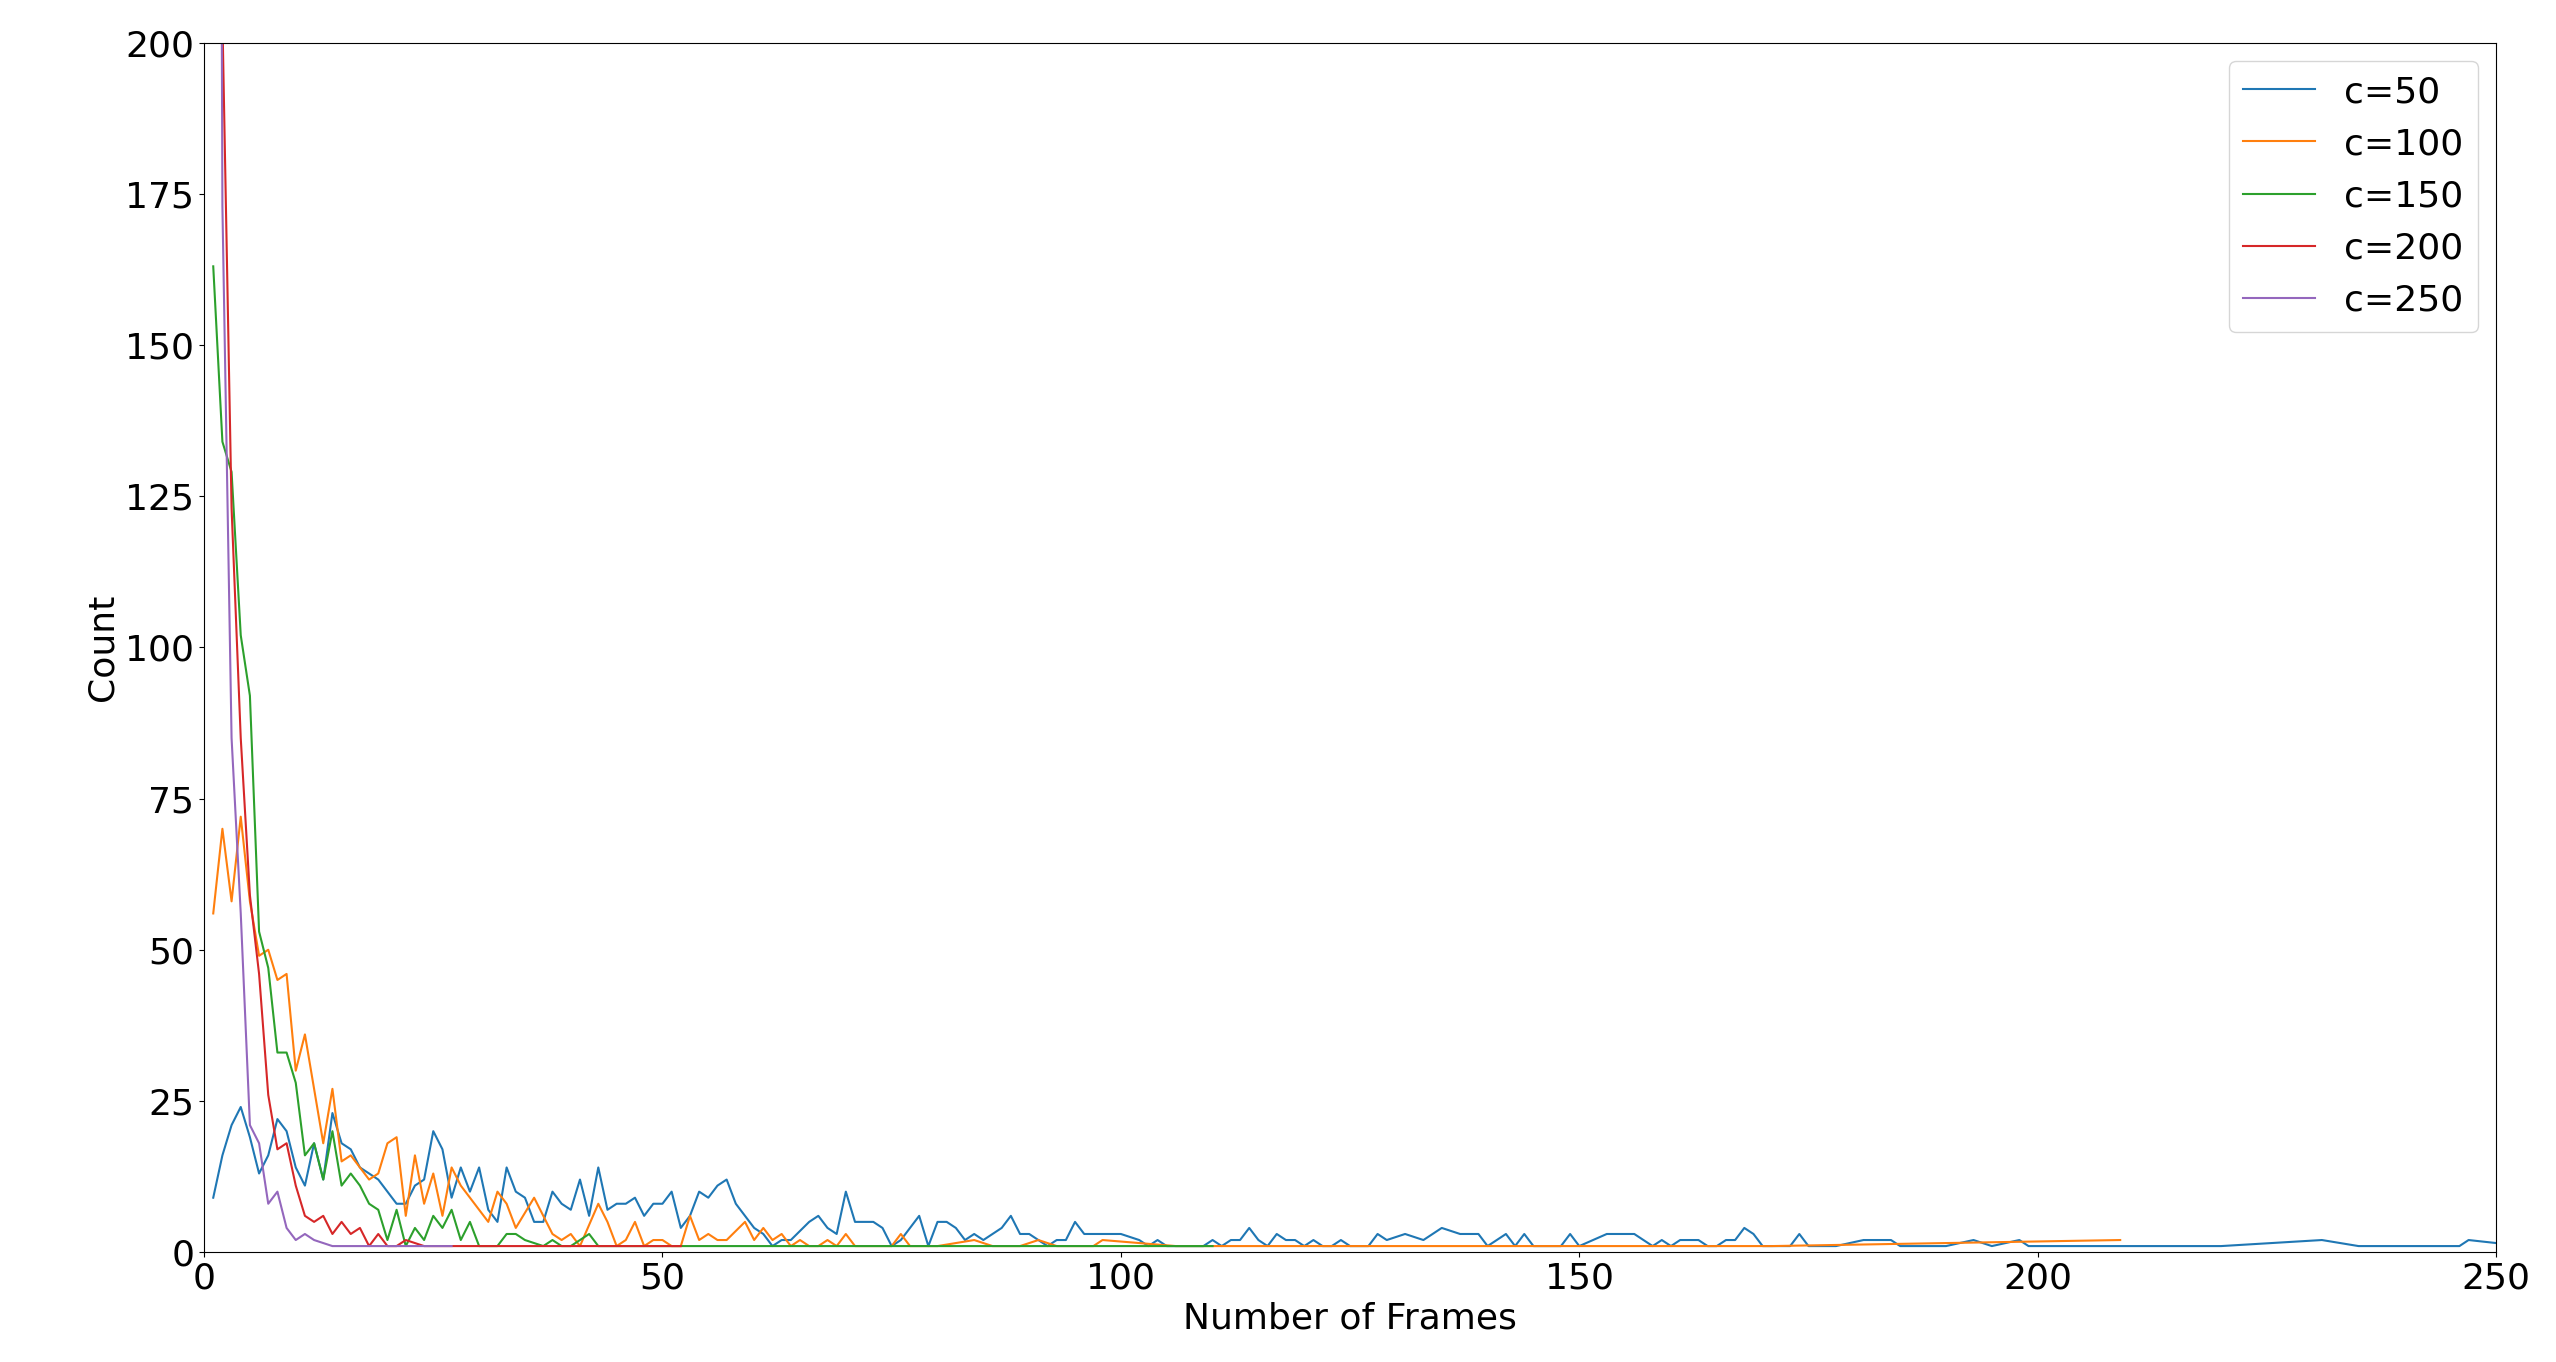
\includegraphics[width=0.8\textwidth]{figures/num_frames_histogram.png}
      \caption{Number of frames selected per video in the MSR-VTT dataset retrieval split when using greedy L1 selection, for different thresholds.}
      \label{fig:optical_flow}
\end{figure}

L1 was chosen over L2 because L2 is very sensitive to large changes in a few pixels; L1 gives a better sense of the overall change in the image.

\section{Prompting Strategies}

The LLM used in testing this pipeline is LLava \cite{llava}.
LLaVA is selected because it is free and open source, and can be run on a single consumer GPU, making it amenable to experimentation.

Beam search, multiple prompts with a temperature.
Two prompts are tried in this work, one of which is is dubbed "concise" (C), while the other is "verbose" (V).
The concise prompt is ""
The verbose prompt is "Please describe the objects in this image. Be as descriptive as possible."
For getting a textual description of a single image, the prompt used is "Please describe the objects in this image. Be as descriptive as possible.".
LLM performance can be sensitive to prompts.

The input to the LLM is a prompt and (potentially) multiple frames, and the output is a text caption.
In all cases, we limit the length of the caption to 512 words, to bound the amount of computation required per frame.

\section{Retrieval}

The last aspect of of the pipeline is, of course, retrieval.
Because LLMs have described the content of the videos at this point in the pipeline, the retrieval task is reduced to that of text retrieval, which is well-studied.
In this work, we explore two retrieval strategies: BM25 and Bi-Encoder, using OpenAI embeddings.
BM25 is a highly performant sparse retriever, relying on term frequencies and other statistics to rank documents.
It is a very fast baseline, retrieving from a thousand documents in milliseconds.

\subsection{Bi-Encoder Retrieval}
This approach is heavily inspired by DPR \cite{dpr}, but uses the same encoder for both documents and queries, and uses L2 distance as a similarity metric instead of the dot product.
In that way, it's similar to the Bi-Encoder strategy used in the BLINK zero-shot entity linker \cite{blink}.
Specifically, the OpenAI model used to generate embedding vectors is \verb|text-embedding-ada-002|, which outputs 1536-dimensional vectors.
The KNN is performed using the FAISS library \cite{faiss}, and all clip descriptions are embedded and stored in an index beforehand, making querying for nearest neighbours very fast.

\begin{figure}
      \centering
      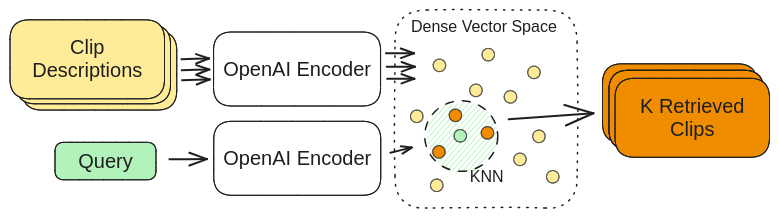
\includegraphics[width=0.8\textwidth]{figures/openai_DPR.png}
      \caption{Bi-Encoder retrieval strategy, using OpenAI embedding API.}
      \label{fig:bienc}
\end{figure}

